\documentclass[conference]{IEEEtran}
\IEEEoverridecommandlockouts

\usepackage{cite}
\usepackage{amsmath,amssymb,amsfonts}
\usepackage{graphicx}
\usepackage{booktabs}
\usepackage{listings}
\usepackage{xcolor}
\usepackage{url}
\usepackage{hyperref}
\usepackage[T1]{fontenc}
\usepackage[utf8]{inputenc}
\usepackage[english]{babel}
\usepackage{tikz}
\usetikzlibrary{arrows.meta, positioning, shapes.geometric, fit, backgrounds}

\graphicspath{{images/}}

\hypersetup{
  colorlinks=true,
  linkcolor=black,
  citecolor=black,
  urlcolor=blue,
}

\begin{document}

\title{HantaBERT: Klasifikasi Multi-Task Hantavirus\\dengan Fine-Tuning DNABERT-2}

\author{%
\IEEEauthorblockN{%
\begin{tabular}{@{}c@{\hspace{2.5em}}c@{\hspace{2.5em}}c@{}}
Muhammad Faiz Atharrahman\textsuperscript{1} &
Muhammad Rafi Dhiyaulhaq\textsuperscript{2} &
Lydia Gracia\textsuperscript{3} \\
18222063 & 18222069 & 18222035
\end{tabular}}
\IEEEauthorblockA{%
Program Studi Sistem dan Teknologi Informasi \\
Sekolah Teknik Elektro dan Informatika \\
Institut Teknologi Bandung \\[2pt]
\textsuperscript{1}\texttt{m@faiz.at} \quad$\cdot$\quad
\textsuperscript{2}\texttt{rafidhiyaulh@gmail.com} \quad$\cdot$\quad
\textsuperscript{3}\texttt{ly.gracies@gmail.com}
}
}

\maketitle

\begin{abstract}
Hantavirus merupakan kelompok virus RNA zoonotik yang ditularkan terutama
oleh rodensia dan mampu menyebabkan demam berdarah berat pada manusia.
Klasifikasi cepat suatu sekuens baru (meliputi spesies virus, kemungkinan
inang reservoir, dan asal geografisnya) merupakan langkah krusial dalam
respons wabah. Penelitian ini mengusulkan \emph{HantaBERT}, sebuah model
multi-task hasil \emph{fine-tuning} terhadap model fondasi genom
\textsc{DNABERT-2} pada 8.822 sekuens hantavirus dari NCBI GenBank.
Arsitektur yang diusulkan menempatkan sebuah \emph{bottleneck} bersama di
atas \emph{encoder} DNABERT-2, then mempercabangkan tiga kepala
klasifikasi independen untuk tugas prediksi spesies (23 kelas), inang
(3 kelas), dan asal geografis (7 benua). Pelatihan dilakukan dengan
\emph{loss} berbobot lintas-tugas $L = 1{,}0\,L_{\text{sp}} + 0{,}5\,L_{\text{host}}
+ 0{,}3\,L_{\text{geo}}$, \emph{learning rate} diferensial encoder-vs-kepala,
serta optimasi memori \emph{gradient accumulation} + AMP fp16. Pada set uji
terpisah, model mencapai akurasi 96{,}7\% (spesies), 91{,}4\% (inang), dan
80{,}5\% (geografi). Visualisasi UMAP atas \emph{embedding bottleneck}
memperlihatkan pemisahan \emph{lineage} virus sekaligus substruktur per
segmen genom ($S$/$M$/$L$) tanpa objektif \emph{clustering} eksplisit,
mengindikasikan terbentuknya representasi filogenetik yang bermakna.
Kode tersedia di \url{https://github.com/HantaBERT}.
\end{abstract}

\begin{IEEEkeywords}
hantavirus, DNABERT-2, multi-task learning, klasifikasi sekuens nukleotida,
embedding genom, UMAP
\end{IEEEkeywords}

% =============================================================================
\section{Pendahuluan}\label{sec:intro}
% =============================================================================

\subsection{Konsep Biologi Hantavirus}

Hantavirus (famili \emph{Hantaviridae}, genus \emph{Orthohantavirus})
adalah virus RNA untai negatif dengan genom tersegmen tiga: segmen
\textbf{S} (\emph{small}, $\sim$1{,}8 kb) mengkodekan protein nukleokapsid
(N) yang membungkus genom; segmen \textbf{M} (\emph{medium}, $\sim$3{,}6 kb)
mengkodekan prekursor glikoprotein yang dipotong menjadi Gn dan Gc
penyusun selubung; dan segmen \textbf{L} (\emph{large}, $\sim$6{,}5 kb)
mengkodekan RNA-\emph{dependent} RNA polimerase (RdRp). Virus ini
ditularkan terutama oleh rodensia, dengan beberapa spesies dapat
menyebabkan dua sindrom klinis berat pada manusia:
\emph{Hantavirus Cardiopulmonary Syndrome} (HCPS) di Amerika dan
\emph{Hemorrhagic Fever with Renal Syndrome} (HFRS) di Eurasia.
Identifikasi cepat sekuens baru menjadi komponen penting respons wabah
dan surveilans epidemiologi.

\subsection{Metode Komputasi Terkait}

Pendekatan klasik berbasis pelurusan (\emph{alignment}) dan pohon
filogenetik (\emph{neighbor-joining}, \emph{maximum likelihood})
memberikan hasil akurat tetapi membutuhkan praproses padat-komputasi dan
sensitif terhadap pemilihan daerah referensi. Pendekatan pembelajaran
mendalam menghadirkan jalur alternatif: \emph{Convolutional Neural Network}
(CNN) untuk klasifikasi taksonomi virus dan, lebih mutakhir, model fondasi
Transformer untuk sekuens nukleotida. \textsc{DNABERT}~\cite{Ji2021DNABERT}
melatih \emph{encoder} BERT~\cite{Devlin2019BERT} pada genom manusia
dengan tokenisasi $k$-\emph{mer}; \textsc{DNABERT-2}~\cite{Zhou2023DNABERT2}
memperluasnya ke multi-spesies dengan tokenisasi \emph{Byte-Pair Encoding}
yang lebih efisien; \textsc{DNABERT-S}~\cite{Zhou2024DNABERTS} menambahkan
fungsi tujuan \emph{species-aware} pada tahap pra-pelatihan.
\emph{Multi-task learning} sendiri telah lama dikenal sebagai bentuk
regularisasi implisit~\cite{Caruana1997MTL}, dan \textsc{UMAP}~\cite{McInnes2018UMAP}
banyak dipakai untuk memvisualkan \emph{embedding} berdimensi tinggi
secara nonlinier.

\subsection{Rumusan Pertanyaan Penelitian}

Penelitian ini berangkat dari tiga pertanyaan:
\begin{description}
  \item[\textbf{RQ1}] Sejauh mana \emph{fine-tuning} multi-task
        DNABERT-2 dengan satu \emph{bottleneck} bersama mampu menghasilkan
        akurasi kompetitif pada tiga atribut hantavirus (spesies, inang,
        geografi) secara simultan?
  \item[\textbf{RQ2}] Apakah \emph{embedding} keluaran \emph{bottleneck}
        merefleksikan struktur filogenetik virus, meskipun model tidak
        pernah dilatih dengan objektif \emph{clustering} eksplisit?
  \item[\textbf{RQ3}] Sifat biologis apa yang muncul dari analisis
        substruktur intra-spesies pada \emph{embedding} tersebut?
\end{description}

\subsection{Kontribusi}

Kontribusi penelitian ini diringkas sebagai berikut:
\begin{itemize}
  \item Mengusulkan \emph{HantaBERT}: arsitektur multi-task yang
        membungkus DNABERT-2 dengan \emph{bottleneck} bersama dan tiga
        kepala klasifikasi independen untuk spesies, inang, dan geografi.
  \item Mendesain \emph{loss} multi-task berbobot dengan bobot kelas
        \emph{balanced} untuk menangani ketimpangan distribusi
        \emph{lineage} hantavirus yang ekstrim.
  \item Melaporkan akurasi 96{,}7\%/91{,}4\%/80{,}5\% pada set uji
        terpisah dan menunjukkan bahwa \emph{embedding bottleneck} secara
        spontan membentuk klaster lineage \emph{plus} substruktur per
        segmen genom ($S$/$M$/$L$).
  \item Membuka kode sumber, hiperparameter, dan skrip evaluasi di
        \url{https://github.com/HantaBERT} untuk reproduksi dan
        eksperimen lanjut.
  \item Mengembangkan antarmuka web publik berbasis FastAPI + HTML/JS
        statis yang membungkus model siap-pakai untuk inferensi
        interaktif: input sekuens DNA/RNA atau berkas FASTA, keluaran
        prediksi probabilistik per tugas dengan \emph{top-N ranking}
        dan visualisasi peta geografis.
\end{itemize}

% =============================================================================
\section{Metode}\label{sec:method}
% =============================================================================

\subsection{Dataset dan Pra-pemrosesan}

Kumpulan data dasar disusun dari pengajuan hantavirus pada NCBI GenBank
dan diolah lewat pipa internal. Setiap baris memuat sekuens nukleotida,
label segmen ($S$/$M$/$L$), label spesies, label inang
(\emph{Rodent}/\emph{Human}/\emph{Others}/\emph{Unknown}), and koordinat
geografis bila tersedia. Sekuens disimpan dalam representasi DNA
($T$, bukan $U$) sehingga dapat langsung diberikan kepada \emph{tokenizer}
DNABERT-2.

Kolom \emph{geo\_label\_broad} sumber menunjukkan tingkat ketidaklengkapan yang luas dan
diperbaiki melalui \emph{reverse geocoding} batch atas pasangan
latitude/longitude. Hasil pemetaan kode negara ke benua menggunakan tabel
\texttt{CC\_TO\_CONTINENT} memberi tujuh kelas (Amerika, Eropa, Asia,
Afrika, Oseania, Lainnya, \emph{Unknown}). Spesies dengan $<\!30$ sampel
digabungkan menjadi kelas \emph{Other}, entri \emph{Orthohantavirus sp.}
dibuang, dan 579 baris inang \emph{Unknown} dihapus. Data dibagi
stratifikasi pada label spesies (80/10/10) menjadi 7.057/882/883
sekuens (Tabel~\ref{tab:dataset}). Bobot kelas dihitung dengan strategi
\emph{balanced} dari \texttt{sklearn} untuk setiap tugas.

\begin{table}[t]
\centering
\caption{Komposisi kumpulan data setelah pra-pemrosesan.}
\label{tab:dataset}
\begin{tabular}{lc|lcc}
\toprule
\textbf{Subset} & \textbf{N seq.} &
\textbf{Tugas} & \textbf{Kelas} & \textbf{Bobot} \\
\midrule
Train & 7.057 & Spesies  & 23 & \emph{balanced} \\
Val   & 882   & Inang    & 3  & \emph{balanced} \\
Test  & 883   & Geografi & 7  & \emph{balanced} \\
\midrule
\textbf{Total} & \textbf{8.822} & & & \\
\bottomrule
\end{tabular}
\end{table}

\subsection{Arsitektur HantaBERT}

HantaBERT terdiri atas tiga komponen utama: \emph{encoder} DNABERT-2
pra-latih, satu lapisan \emph{bottleneck} bersama, dan tiga kepala
klasifikasi independen. Bagan alir komputasinya disajikan pada
Gambar~\ref{fig:flow}. Diberikan masukan sekuens nukleotida sepanjang
maksimum $L_{\max}=512$ token BPE, alur komputasinya adalah:
\[
\begin{aligned}
\mathbf{H} &= \text{DNABERT2}(\mathbf{x}) \in \mathbb{R}^{L \times 768}, \\
\mathbf{h} &= \text{MeanPool}(\mathbf{H}, \mathbf{m}) \in \mathbb{R}^{768}, \\
\mathbf{z} &= \text{Dropout}(\text{GELU}(\text{LayerNorm}(W\mathbf{h}\!+\!b))), \\
\mathbf{y}_{\text{task}} &= W_{\text{task}}\,\text{Dropout}(\mathbf{z}) + b_{\text{task}},
\quad \text{task} \in \{\text{sp},\text{host},\text{geo}\}.
\end{aligned}
\]
\emph{Mean pooling} dihitung sebagai rerata berbobot \emph{attention mask}
\(
\mathbf{h} = \sum_i m_i \mathbf{H}_i / \max(\sum_i m_i, \varepsilon)
\)
sehingga token \emph{padding} tidak ikut diperhitungkan. \emph{Bottleneck}
$W \in \mathbb{R}^{768\times 768}$ bersifat \emph{task-agnostic}:
parameternya dilatih oleh ketiga tugas sekaligus, memaksa representasi
$\mathbf{z}$ memuat informasi yang berguna bagi semua tugas. Tiap kepala
memiliki \emph{dropout} independen $0{,}1$ sebelum lapisan linier akhir
untuk meredam interferensi gradien antar-tugas.

\begin{figure}[t]
\centering
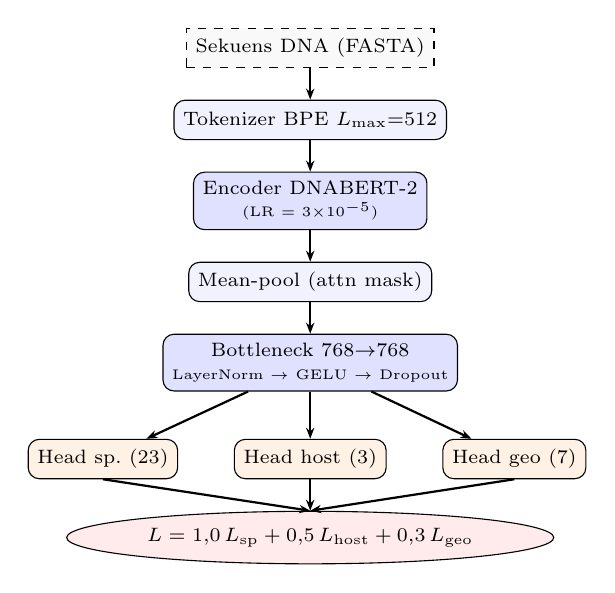
\begin{tikzpicture}[
  node distance=4mm and 6mm,
  every node/.style={font=\scriptsize},
  block/.style={rectangle, draw, rounded corners, minimum width=2.2cm,
                minimum height=5mm, align=center, fill=blue!5},
  data/.style={rectangle, draw, dashed, minimum width=2.2cm,
               minimum height=5mm, align=center, fill=gray!5},
  head/.style={rectangle, draw, rounded corners, minimum width=1.7cm,
               minimum height=5mm, align=center, fill=orange!10},
  loss/.style={ellipse, draw, minimum width=1.6cm, minimum height=5mm,
               align=center, fill=red!8},
  arrow/.style={-{Stealth[length=1.4mm]}, thick},
]
\node[data] (seq) {Sekuens DNA (FASTA)};
\node[block, below=of seq] (tok) {Tokenizer BPE $L_{\max}{=}512$};
\node[block, below=of tok, fill=blue!12] (enc)
      {Encoder DNABERT-2 \\ \tiny (LR = $3{\times}10^{-5}$)};
\node[block, below=of enc] (pool) {Mean-pool (attn mask)};
\node[block, below=of pool, fill=blue!12] (bot)
      {Bottleneck $768{\to}768$ \\ \tiny LayerNorm $\to$ GELU $\to$ Dropout};
\node[head, below left=6mm and -2mm of bot]  (hsp)  {Head sp.\ (23)};
\node[head, below=6mm of bot]                (hho)  {Head host (3)};
\node[head, below right=6mm and -2mm of bot] (hge)  {Head geo (7)};
\node[loss, below=of hho] (loss) {$L = 1{,}0\,L_{\text{sp}} + 0{,}5\,L_{\text{host}} + 0{,}3\,L_{\text{geo}}$};
\draw[arrow] (seq)  -- (tok);
\draw[arrow] (tok)  -- (enc);
\draw[arrow] (enc)  -- (pool);
\draw[arrow] (pool) -- (bot);
\draw[arrow] (bot)  -- (hsp);
\draw[arrow] (bot)  -- (hho);
\draw[arrow] (bot)  -- (hge);
\draw[arrow] (hsp.south) -- (loss.north);
\draw[arrow] (hho.south) -- (loss.north);
\draw[arrow] (hge.south) -- (loss.north);
\end{tikzpicture}
\caption{Bagan alir HantaBERT. Komponen biru-tua dilatih dengan
\emph{learning rate} encoder ($3\!\times\!10^{-5}$); komponen biru muda
dan oranye dengan LR sepuluh kali lebih besar.}
\label{fig:flow}
\end{figure}

\subsection{Fungsi \emph{Loss} Multi-Task}

\emph{Loss} keseluruhan adalah kombinasi linier dari tiga
\emph{cross-entropy} terbobot kelas:
\[
L \;=\; \lambda_{\text{sp}}\,L_{\text{sp}}
     \,+\, \lambda_{\text{host}}\,L_{\text{host}}
     \,+\, \lambda_{\text{geo}}\,L_{\text{geo}},
\]
dengan $\lambda_{\text{sp}}{=}1{,}0$, $\lambda_{\text{host}}{=}0{,}5$,
dan $\lambda_{\text{geo}}{=}0{,}3$. Bobot mencerminkan prioritas relatif:
spesies adalah tugas utama dengan supervisi terbersih, sementara geografi
memiliki rasio sinyal-derau terendah.

\subsection{Strategi Pelatihan}

Konfigurasi pelatihan diringkas pada Tabel~\ref{tab:hyper}. \emph{Encoder}
pra-latih diberi laju pembelajaran sepuluh kali lebih kecil dibanding
lapisan baru (\emph{bottleneck} dan kepala). Karena \emph{full attention}
512-token DNABERT-2 tidak menampung \emph{batch} 16 pada GPU
\emph{consumer-grade}, \emph{batch size} efektif 16 dicapai melalui
$\text{BATCH\_SIZE}{=}4$ dan $\text{GRAD\_ACCUM\_STEPS}{=}4$. Selain itu,
parameter \texttt{attention\_probs\_dropout\_prob} disetel ke $0{,}1$
untuk memaksa jalur \emph{attention} PyTorch standar, menghindari
\emph{kernel} Triton DNABERT-2 yang melampaui batas \emph{shared memory}.

\begin{table}[t]
\centering
\caption{Hiperparameter pelatihan utama.}
\label{tab:hyper}
\begin{tabular}{ll}
\toprule
\textbf{Parameter} & \textbf{Nilai} \\
\midrule
Backbone & \texttt{zhihan1996/DNABERT-2-117M} \\
Panjang token maks. & 512 BPE \\
\emph{Batch size} & 4 ($\times$ 4 \emph{grad accum} = efektif 16) \\
LR encoder / kepala & $3{\times}10^{-5}$ / $3{\times}10^{-4}$ \\
Optimasi & AdamW, $\beta=(0{,}9,0{,}999)$, $\text{wd}=0{,}01$ \\
\emph{Warmup} / total epoch & 200 langkah linier / 10 \\
\emph{Mixed precision} & AMP fp16 \\
\emph{Grad clipping} & 1{,}0 (\emph{global norm}) \\
$\lambda_{\text{sp/host/geo}}$ & $1{,}0/0{,}5/0{,}3$ \\
\bottomrule
\end{tabular}
\end{table}

\subsection{Antarmuka Web untuk Inferensi}\label{sec:webui}

Agar model siap digunakan oleh peneliti non-pemrogram, dikembangkan
sebuah antarmuka web publik. Sisi \emph{backend} (\texttt{HantaBERT-API})
membungkus \emph{checkpoint} \texttt{MultiTaskHantaBERT} di balik
layanan FastAPI + Uvicorn, dikemas sebagai \emph{container} Docker
berbasis \texttt{python:3.11-slim}, dan di-\emph{deploy} pada
\texttt{hantabert-api.faizath.com}. Sisi \emph{frontend}
(\texttt{HantaBERT-Web}) berupa berkas statis HTML/CSS/JavaScript murni
tanpa \emph{framework} JS; peta dunia interaktif untuk asal geografis
digambar memakai pustaka D3 dan TopoJSON yang dimuat dari CDN.

Pengguna dapat menempel sekuens DNA/RNA mentah atau mengunggah berkas
FASTA; basa $U$ pada masukan RNA dikonversi otomatis ke $T$ sebelum
tokenisasi BPE, dan sistem menampilkan peringatan ketika sekuens
melampaui 512 token sehingga ter-truncate. Jumlah hasil \emph{top-N}
(1 sampai 23) dapat diatur per tugas, lengkap dengan \emph{confidence score}
yang dapat diperluas. Gambar~\ref{fig:webui} menampilkan keluaran
sistem untuk sekuens uji 224 bp yang dijalankan langsung pada
antarmuka.

\begin{figure}[t]
\centering
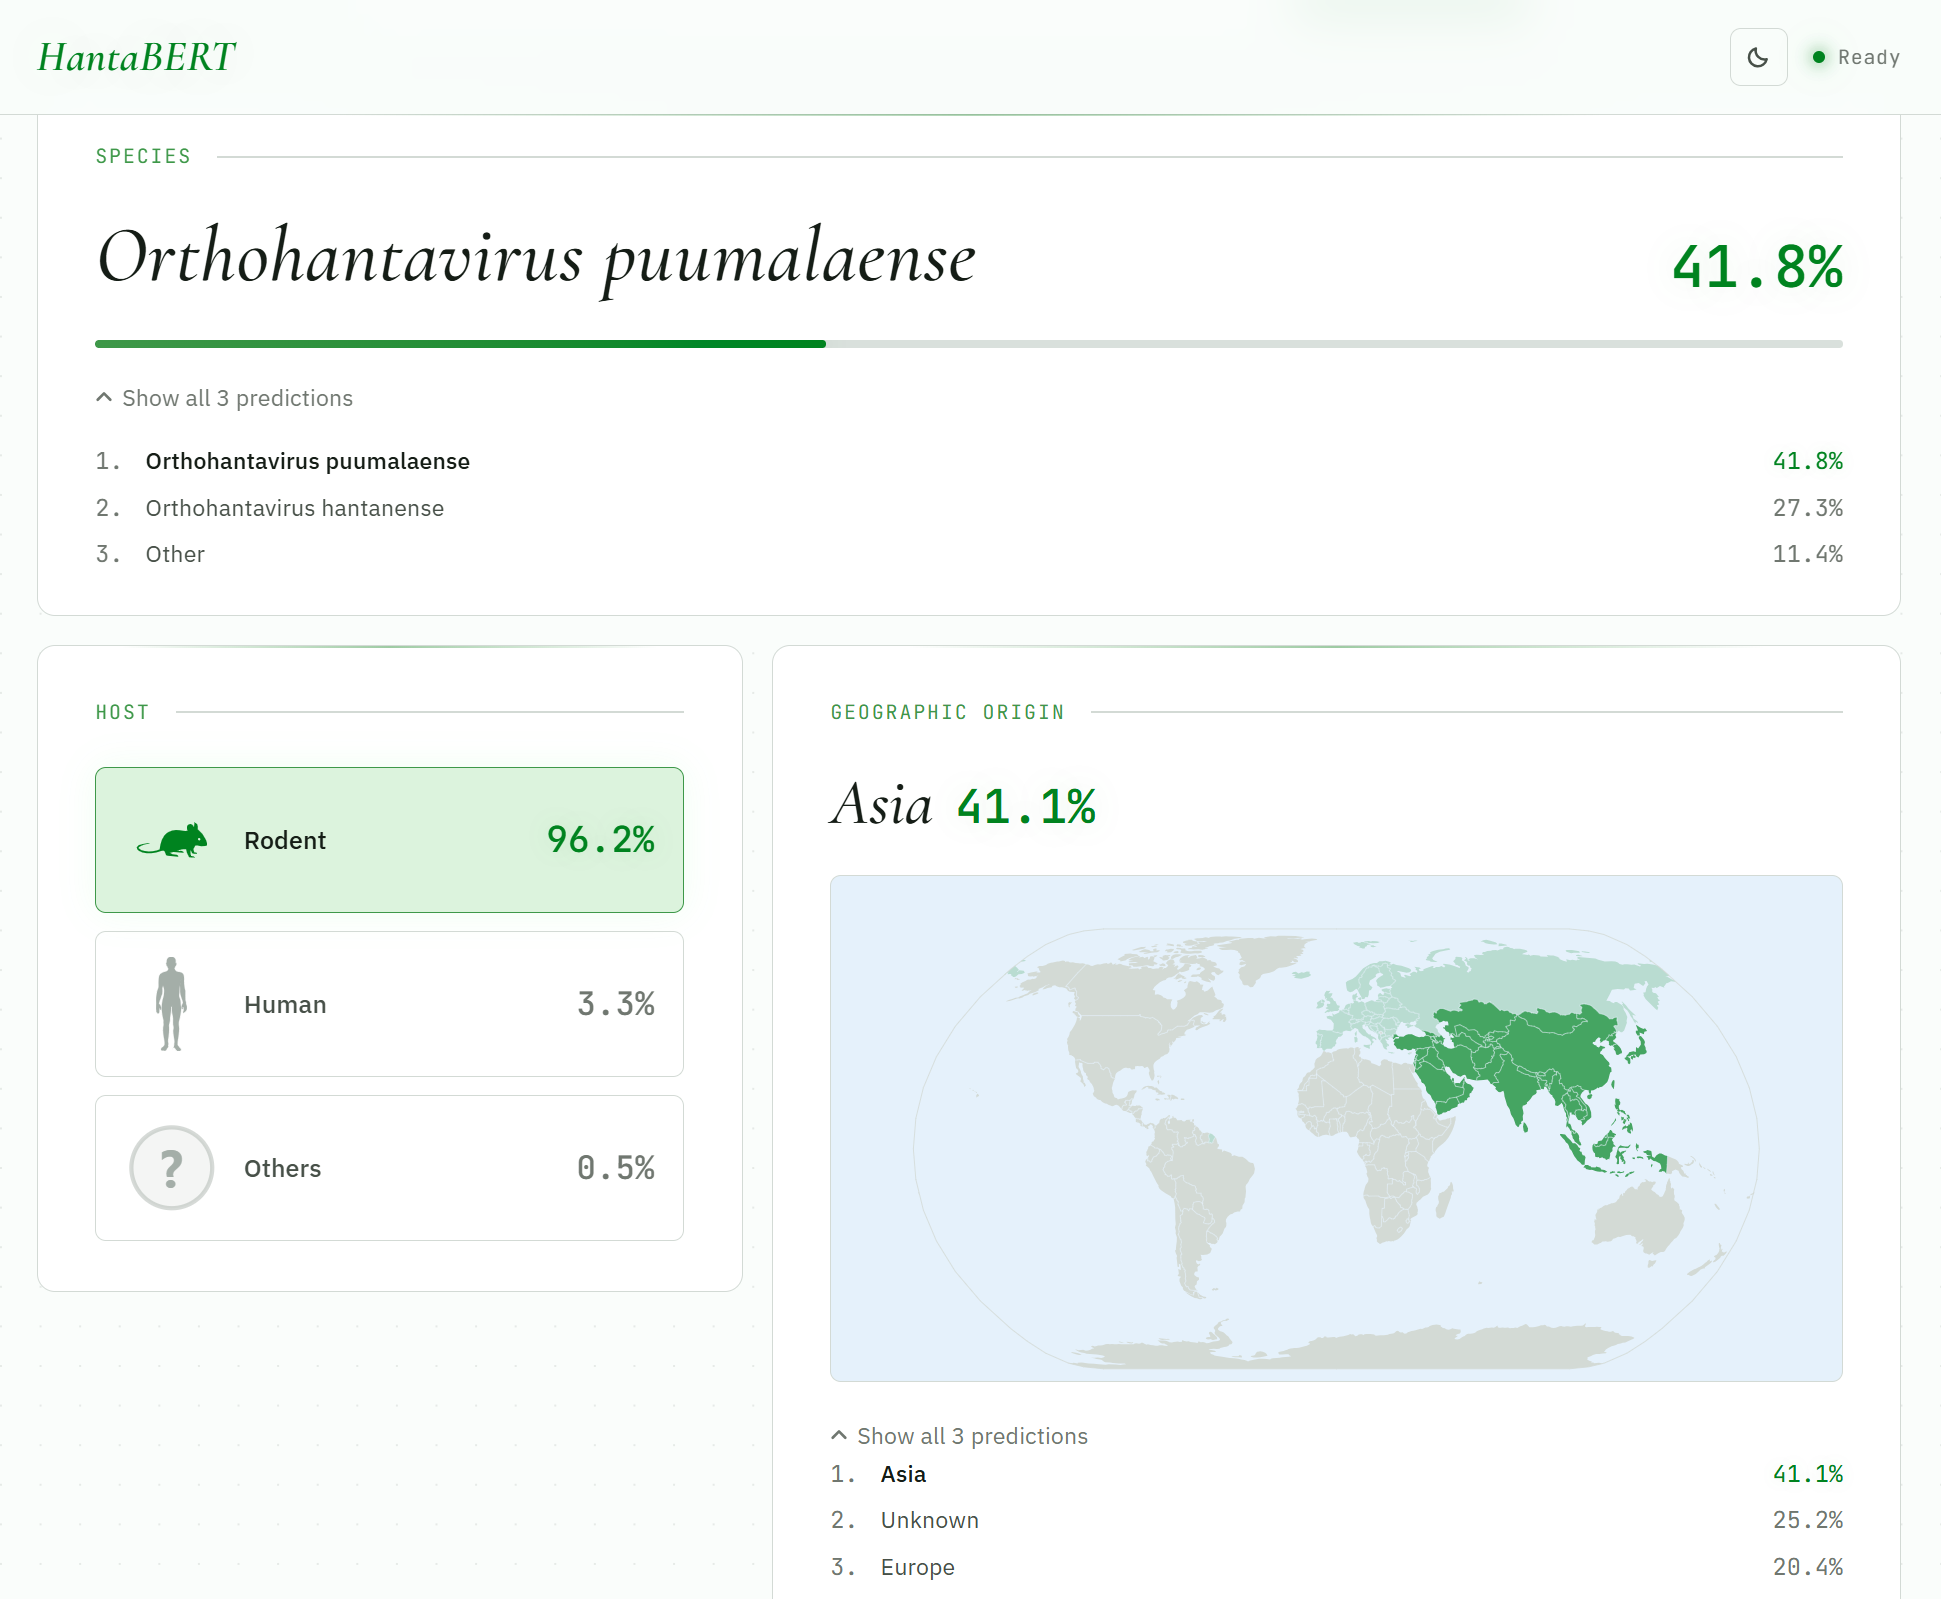
\includegraphics[width=\linewidth]{website-interface.png}
\caption{Tangkapan layar antarmuka web HantaBERT untuk sekuens uji
  224 bp \texttt{ATGAAAGACCTTCTGAAG\ldots GAGAAGCTGGAG}. Prediksi
  \emph{top-1}: \emph{Orthohantavirus puumalaense} ($41{,}8\%$), inang
  \emph{Rodent} ($96{,}2\%$), dan wilayah geografis Asia ($41{,}1\%$).
  Probabilitas \emph{top-3} dapat diperluas pada setiap kartu tugas;
  hasil geografi divisualisasikan pada peta dunia interaktif.}
\label{fig:webui}
\end{figure}

\subsection{Ketersediaan Kode dan Data}

Seluruh artefak dirilis terbuka di organisasi GitHub
\url{https://github.com/HantaBERT}, terdiri dari tiga repositori:
(i) \texttt{HantaBERT}: kode \emph{preprocess}, \emph{train},
\emph{evaluate}, \emph{visualize}, hiperparameter, dan \emph{checkpoint}
model; (ii) \texttt{HantaBERT-API}: layanan inferensi FastAPI
beserta \emph{Dockerfile}; (iii) \texttt{HantaBERT-Web}: berkas
\emph{frontend} statis. Setiap repositori menyertakan
\texttt{requirements.txt}/\texttt{README} berisi versi paket yang teruji
serta panduan reproduksi tahap demi tahap. Selain itu, tautan rekaman video
presentasi disediakan pada \url{https://youtu.be/4Ia0FM7iYb4} dan salindia
presentasi dapat diakses melalui \url{https://canva.link/33nwtodm1si8nxw}.

% =============================================================================
\section{Hasil dan Diskusi}\label{sec:results}
% =============================================================================

\subsection{Progres Pelatihan}

Tabel~\ref{tab:hist} memperlihatkan progres tiap epoch pada set validasi.
Setelah 10 epoch, \emph{val\_loss} turun dari $2{,}443$ menjadi $0{,}797$
dan akurasi validasi mencapai $96{,}7\%$ (spesies), $91{,}4\%$ (inang),
$80{,}5\%$ (geografi). Tugas spesies paling cepat menuju saturasi, sesuai
dengan supervisi terbersih dan jumlah kelas yang membuat sinyal
diskriminatif kaya. Kurva pada Gambar~\ref{fig:curves} menunjukkan
selisih \emph{loss} pelatihan-validasi yang mengecil seiring epoch
tanpa tanda kelebihan pas (*overfitting*) jelas.

\begin{table}[t]
\centering
\caption{Progres pelatihan pada set validasi (10 epoch).}
\label{tab:hist}
\begin{tabular}{cccccc}
\toprule
\textbf{Ep} & \textbf{$L_{\text{tr}}$} & \textbf{$L_{\text{val}}$} &
\textbf{Sp.} & \textbf{Host} & \textbf{Geo} \\
\midrule
1  & 3{,}024 & 2{,}443 & 78{,}9\% & 72{,}8\% & 72{,}3\% \\
3  & 1{,}034 & 1{,}195 & 92{,}9\% & 83{,}1\% & 74{,}1\% \\
5  & 0{,}634 & 1{,}150 & 94{,}0\% & 87{,}1\% & 77{,}6\% \\
7  & 0{,}452 & 0{,}869 & 96{,}5\% & 90{,}4\% & 78{,}1\% \\
9  & 0{,}336 & 0{,}818 & 96{,}3\% & 91{,}4\% & 80{,}3\% \\
\textbf{10} & \textbf{0{,}307} & \textbf{0{,}797} &
\textbf{96{,}7\%} & \textbf{91{,}4\%} & \textbf{80{,}5\%} \\
\bottomrule
\end{tabular}
\end{table}

\begin{figure}[t]
\centering
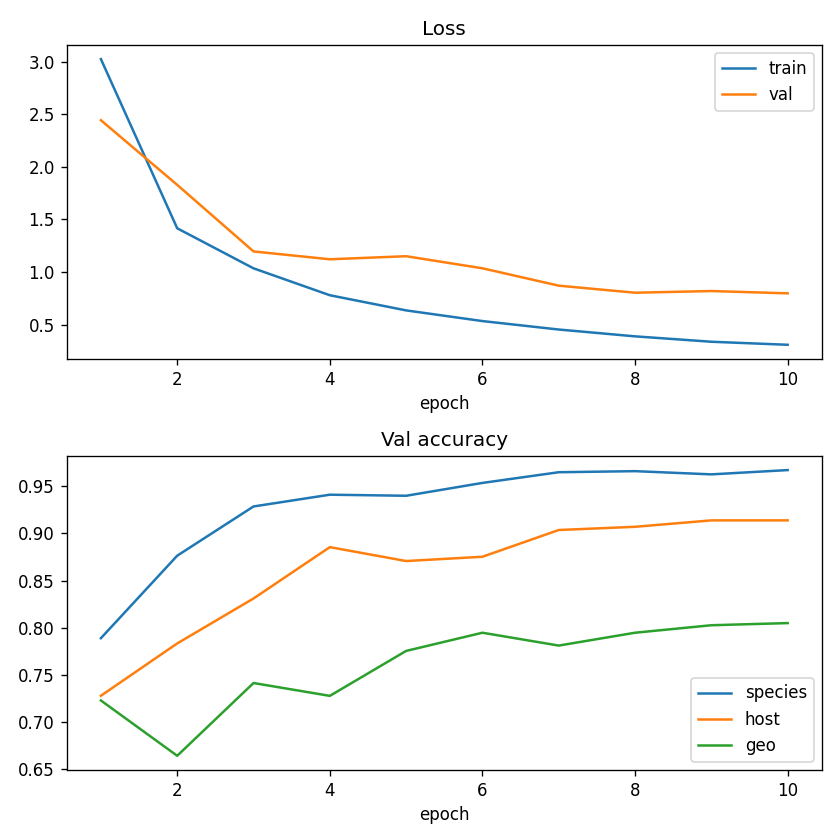
\includegraphics[width=\linewidth]{training_curves.png}
\caption{Kurva \emph{loss} (atas) dan akurasi validasi per tugas (bawah)
selama 10 epoch.}
\label{fig:curves}
\end{figure}

\subsection{Evaluasi pada Set Uji}

Tabel~\ref{tab:test} merangkum akurasi set uji untuk dua jalur evaluasi:
kepala neural pasca-pelatihan dan \emph{baseline} SVM-RBF
($C\!=\!10$, kelas \emph{balanced}) atas \emph{embedding bottleneck}
yang sudah dibekukan dan distandarisasi. Tujuan baseline ini adalah
mengukur kualitas \emph{embedding} secara terisolasi (bukan untuk
mengalahkan kepala neural) dan menjawab \textbf{RQ2}: jika SVM-RBF
sederhana dapat mencapai akurasi tinggi atas $\mathbf{z}$, berarti
\emph{bottleneck} memang telah memetakan sekuens ke ruang yang
kelas-kelasnya terpisah secara non-linier.

\begin{table}[t]
\centering
\caption{Akurasi pada set uji.}
\label{tab:test}
\begin{tabular}{lc}
\toprule
\textbf{Tugas} & \textbf{Kepala neural} \\
\midrule
Spesies (23) & \textbf{96{,}7\%} \\
Inang (3)    & \textbf{91{,}4\%} \\
Geografi (7) & \textbf{80{,}5\%} \\
\bottomrule
\end{tabular}
\end{table}

\subsection{Analisis Kesalahan dan Konteks Biologis}

Gambar~\ref{fig:cm-species} menampilkan \emph{confusion matrix} tugas
spesies; \emph{lineage} dominan (mis. \emph{O.\ seoulense},
\emph{O.\ puumalaense}) terprediksi dengan akurasi yang tinggi, dan kesalahan
terkonsentrasi pada kelas \emph{Other} yang merupakan gabungan lineage
langka, sebuah konsekuensi langsung dari ambang $<\!30$ sampel.

\begin{figure}[t]
\centering
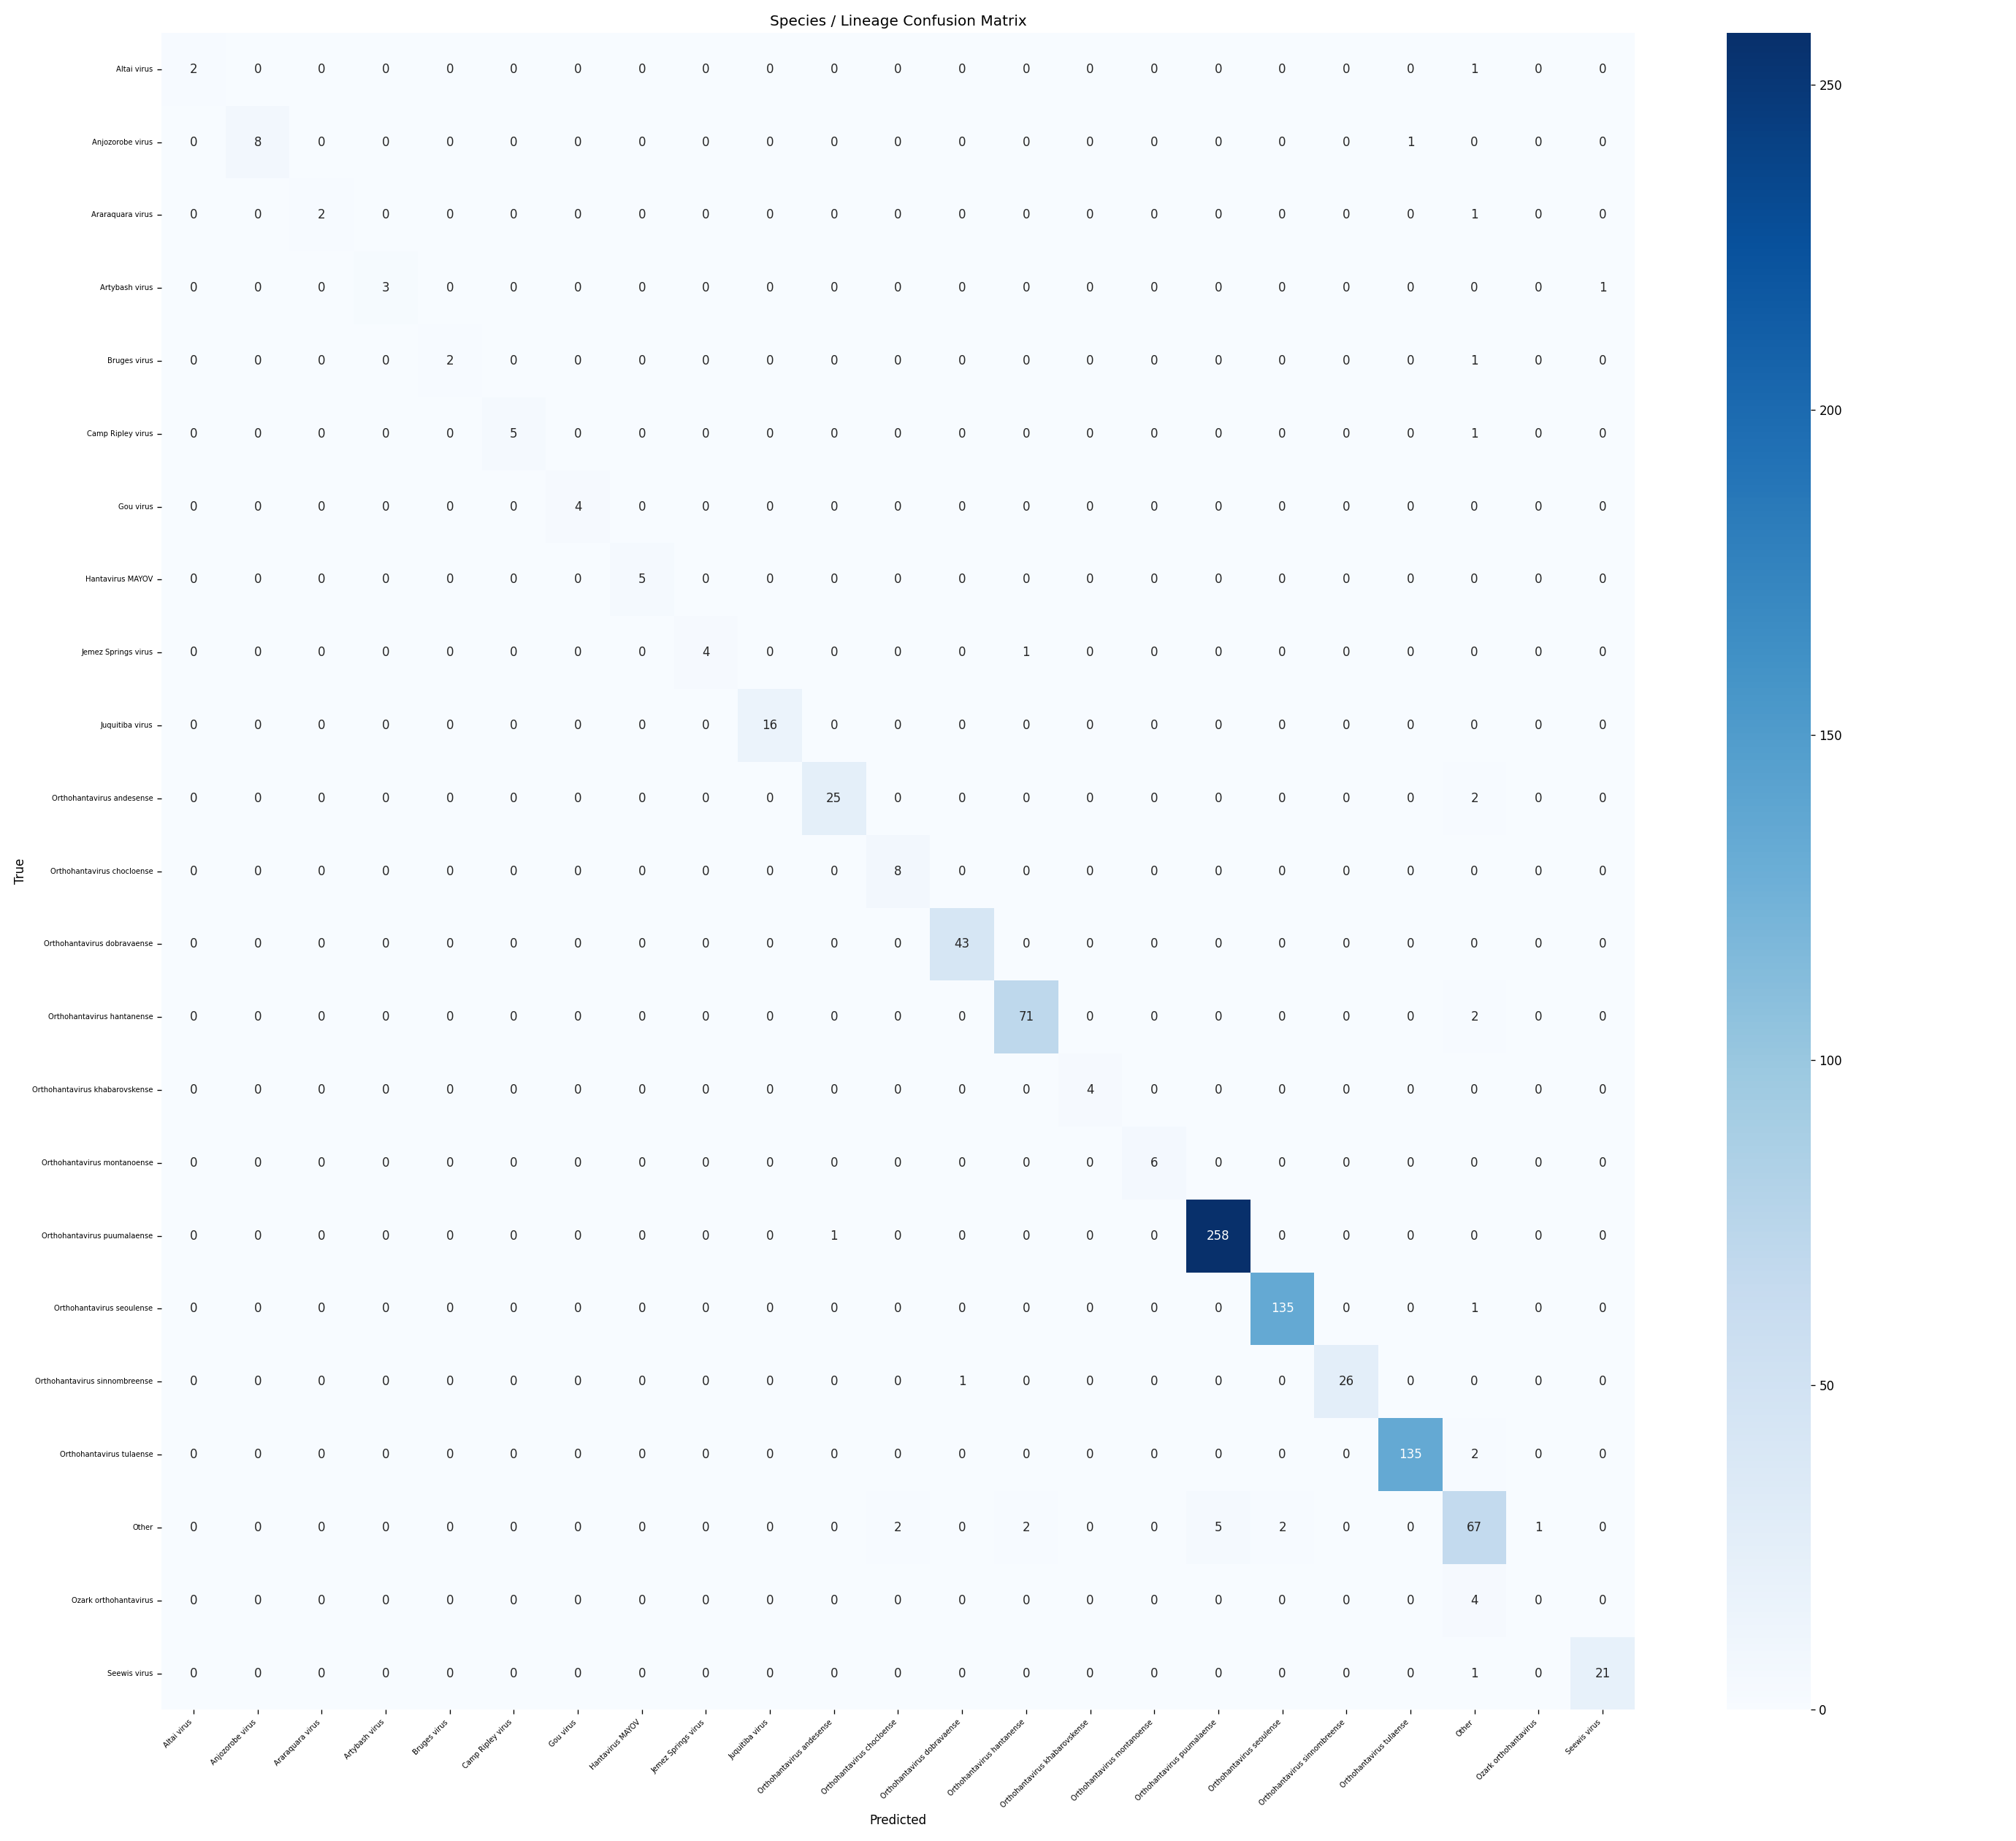
\includegraphics[width=\linewidth]{cm_species.png}
\caption{\emph{Confusion matrix} klasifikasi spesies pada set uji.}
\label{fig:cm-species}
\end{figure}

Pada tugas inang, sebagian besar kesalahan adalah pertukaran antara
\emph{Rodent} dan \emph{Others}, masuk akal karena beberapa hantavirus
(mis. \emph{Thottimvirus}) juga diisolasi dari \emph{Insectivora}
non-rodensia (kelelawar, tikus celurut). Pada tugas geografi,
kesalahan terkonsentrasi pada lineage \emph{kosmopolitan}: Seoul virus
yang dibawa \emph{Rattus norvegicus} ditemukan di semua benua mengikuti
distribusi tikus inangnya, sehingga label benua tidak selalu deterministik
dari sekuens; akurasi $80{,}5\%$ kemungkinan adalah batasan atas
dekat dengan ambiguitas inherent label tersebut.

\subsection{Visualisasi UMAP dan Substruktur Filogenetik}

Untuk menjawab \textbf{RQ2} dan \textbf{RQ3}, UMAP
($n_{\text{neighbors}}{=}20$, $\text{min\_dist}{=}0{,}1$, metrik
\emph{cosine}) diterapkan pada \emph{embedding bottleneck} seluruh
sekuens; varian $n_{\text{neighbors}}{=}15$, $\text{min\_dist}{=}0{,}05$
dipakai untuk plot intra-spesies. Gambar~\ref{fig:umap-all} menunjukkan
\emph{embedding} membentuk klaster terpisah per \emph{lineage}, hasil yang
tidak ter-supervisi secara eksplisit oleh objektif \emph{clustering}.

\begin{figure}[t]
\centering
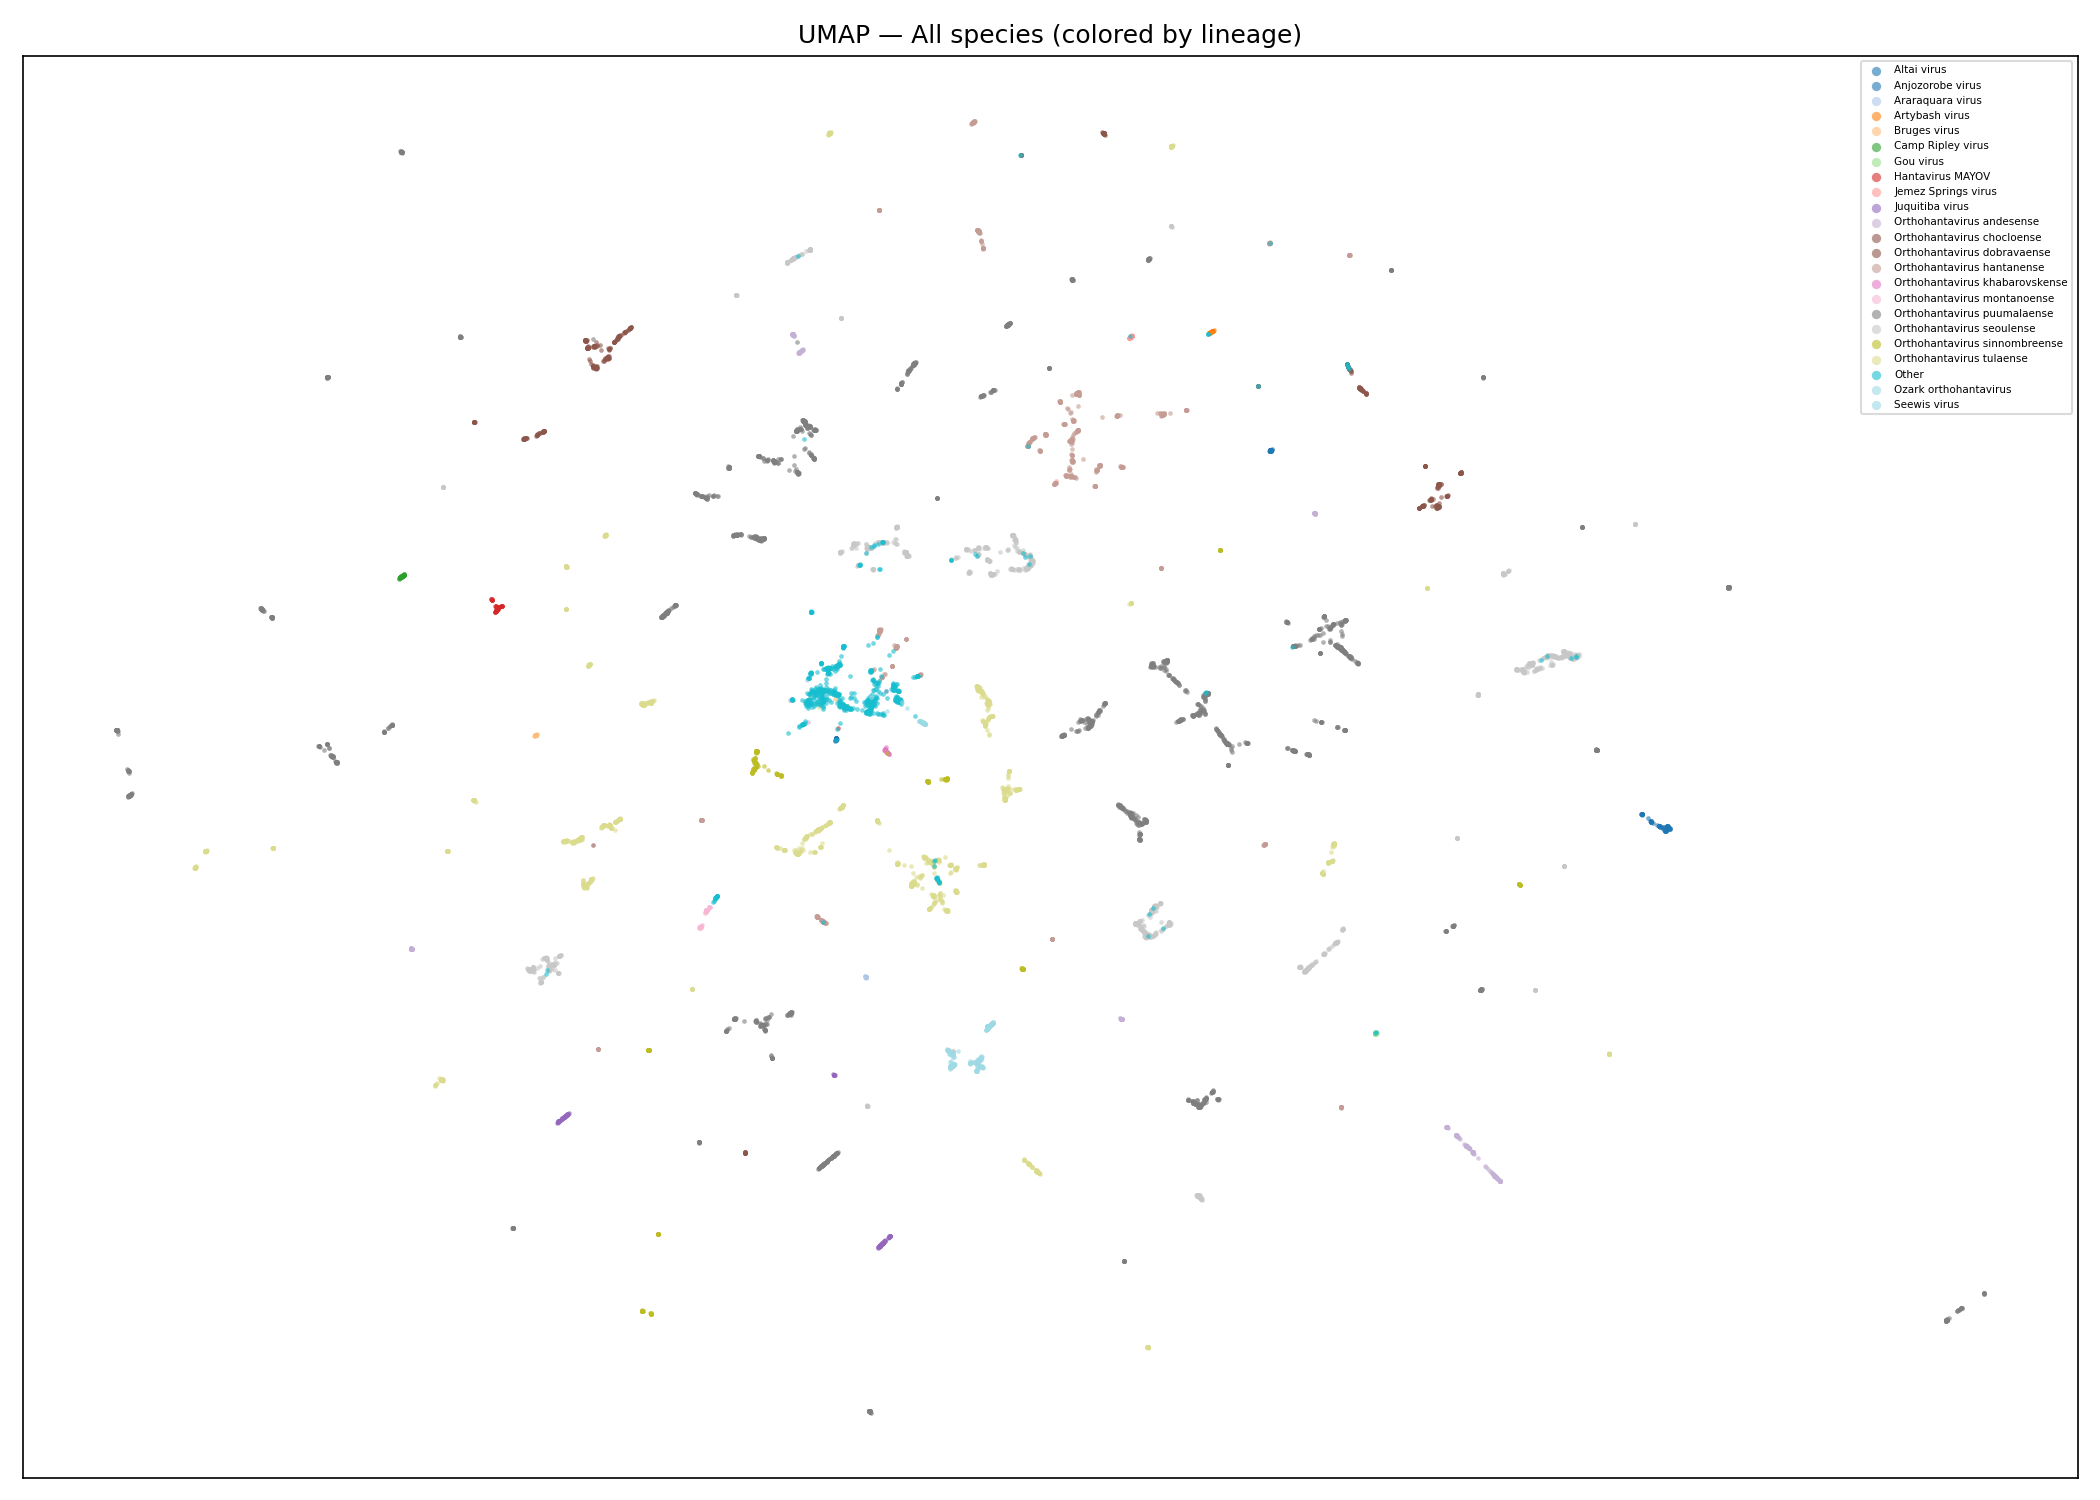
\includegraphics[width=\linewidth]{umap_all_species.png}
\caption{Proyeksi UMAP atas 8.822 sekuens diwarnai per lineage.}
\label{fig:umap-all}
\end{figure}

Plot intra-spesies (Gambar~\ref{fig:umap-seoul} dan~\ref{fig:umap-puumala})
mengungkap fenomena menarik: \emph{embedding} mengelompokkan sekuens
berdasarkan \textbf{segmen genom} ($S$/$M$/$L$) meskipun segmen tidak
pernah menjadi target supervisi. Hal ini konsisten dengan biologi
hantavirus: ketiga segmen mengkodekan protein dengan tekanan selektif dan
kandungan nukleotida yang berbeda: N (segmen S) sangat \emph{conserved},
Gn/Gc (segmen M) mengalami \emph{positive selection} pada situs antigenik
selubung, dan RdRp (segmen L) mempertahankan motif aktif polimerase.
Perbedaan komposisi \emph{di-} dan \emph{tri-nucleotide} ini terdeteksi
oleh \emph{tokenizer} BPE DNABERT-2 dan termanifestasi di
\emph{embedding} sebagai pemisahan klaster, menjawab \textbf{RQ3}: model
secara implisit telah memetakan informasi struktural genom hantavirus.

\begin{figure}[t]
\centering
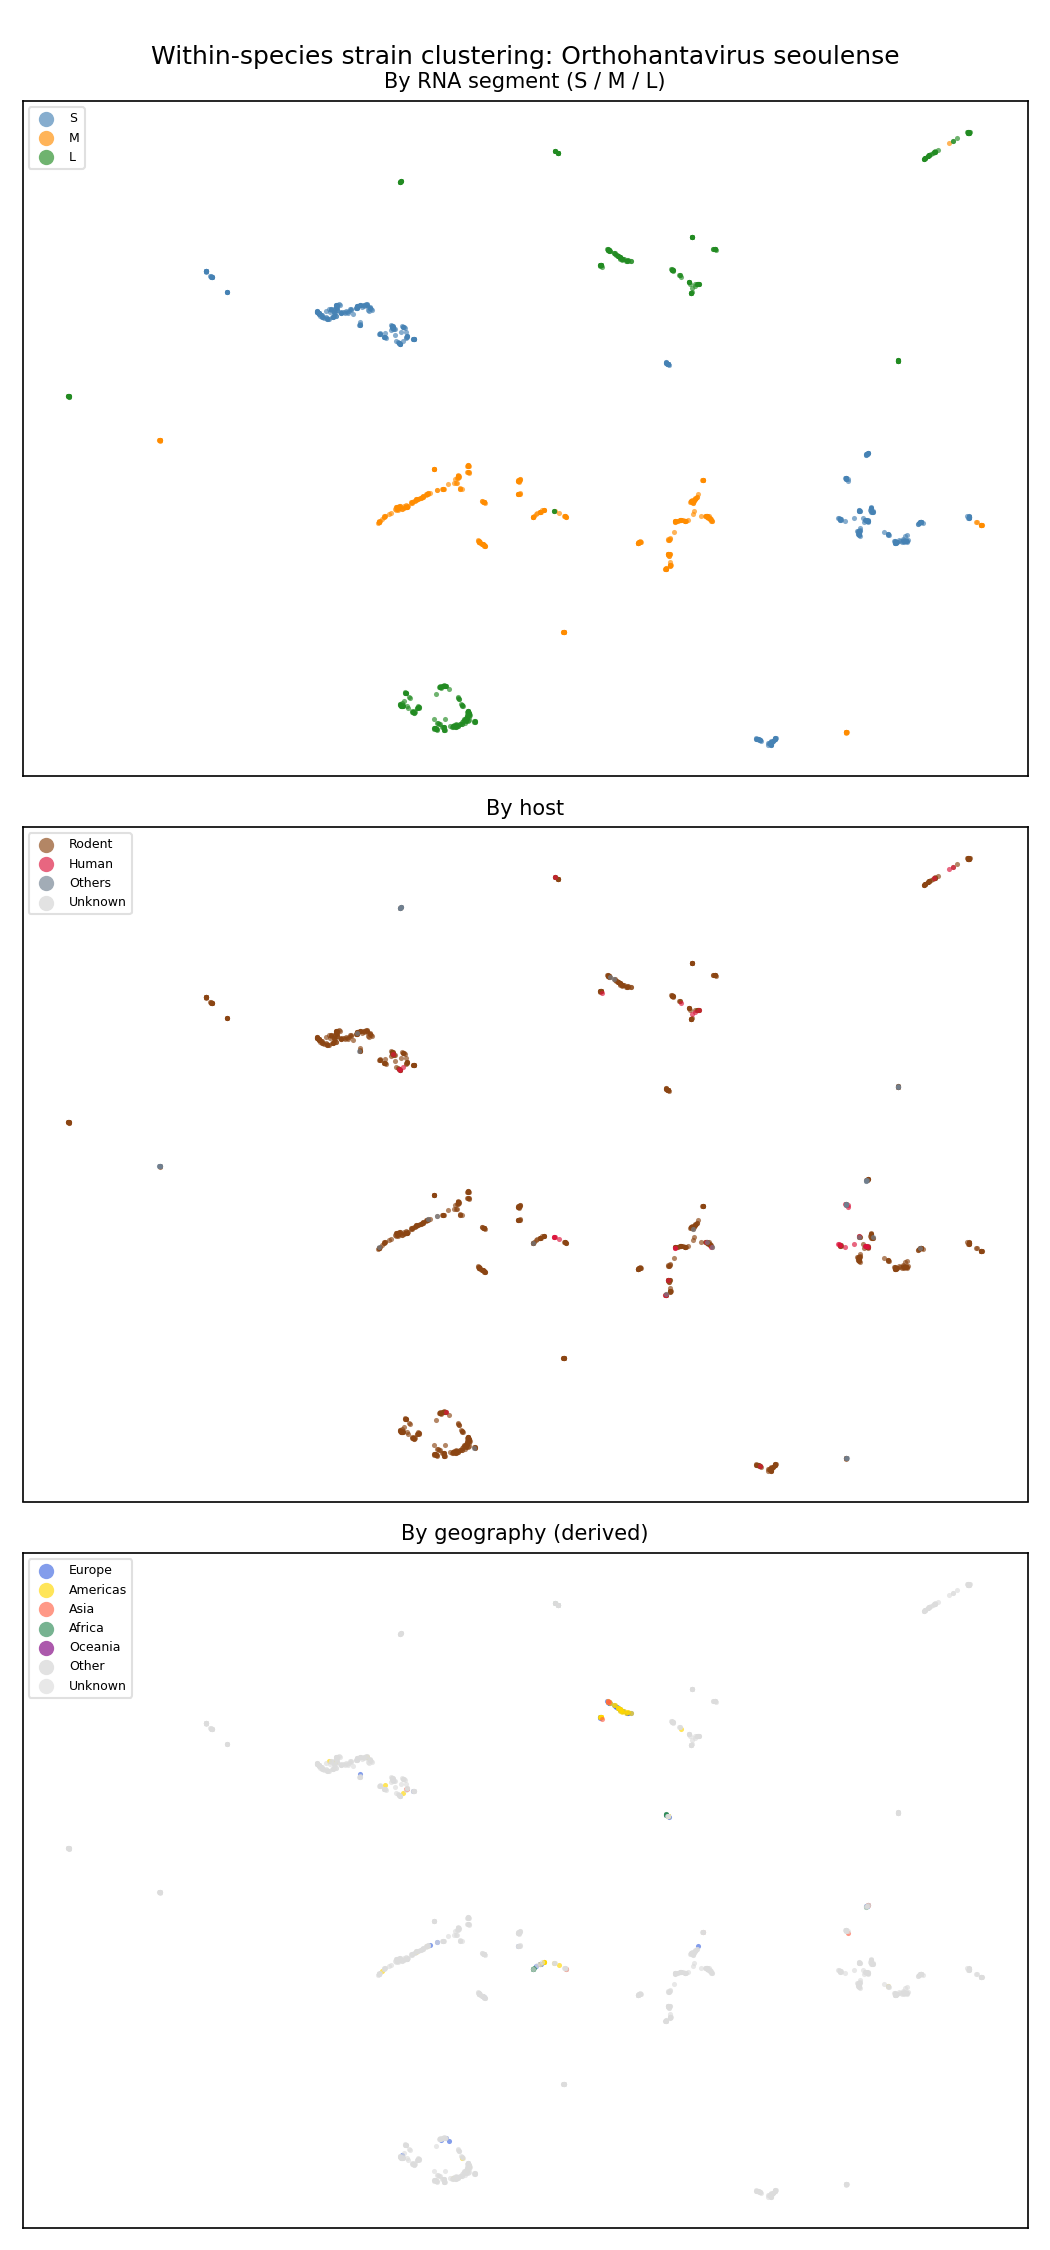
\includegraphics[width=\linewidth,height=0.6\textheight,keepaspectratio]{umap_Orthohantavirus_seoulense.png}
\caption{UMAP intra-spesies \emph{O.\ seoulense} (atas-bawah:
segmen / inang / geografi).}
\label{fig:umap-seoul}
\end{figure}

\begin{figure}[t]
\centering
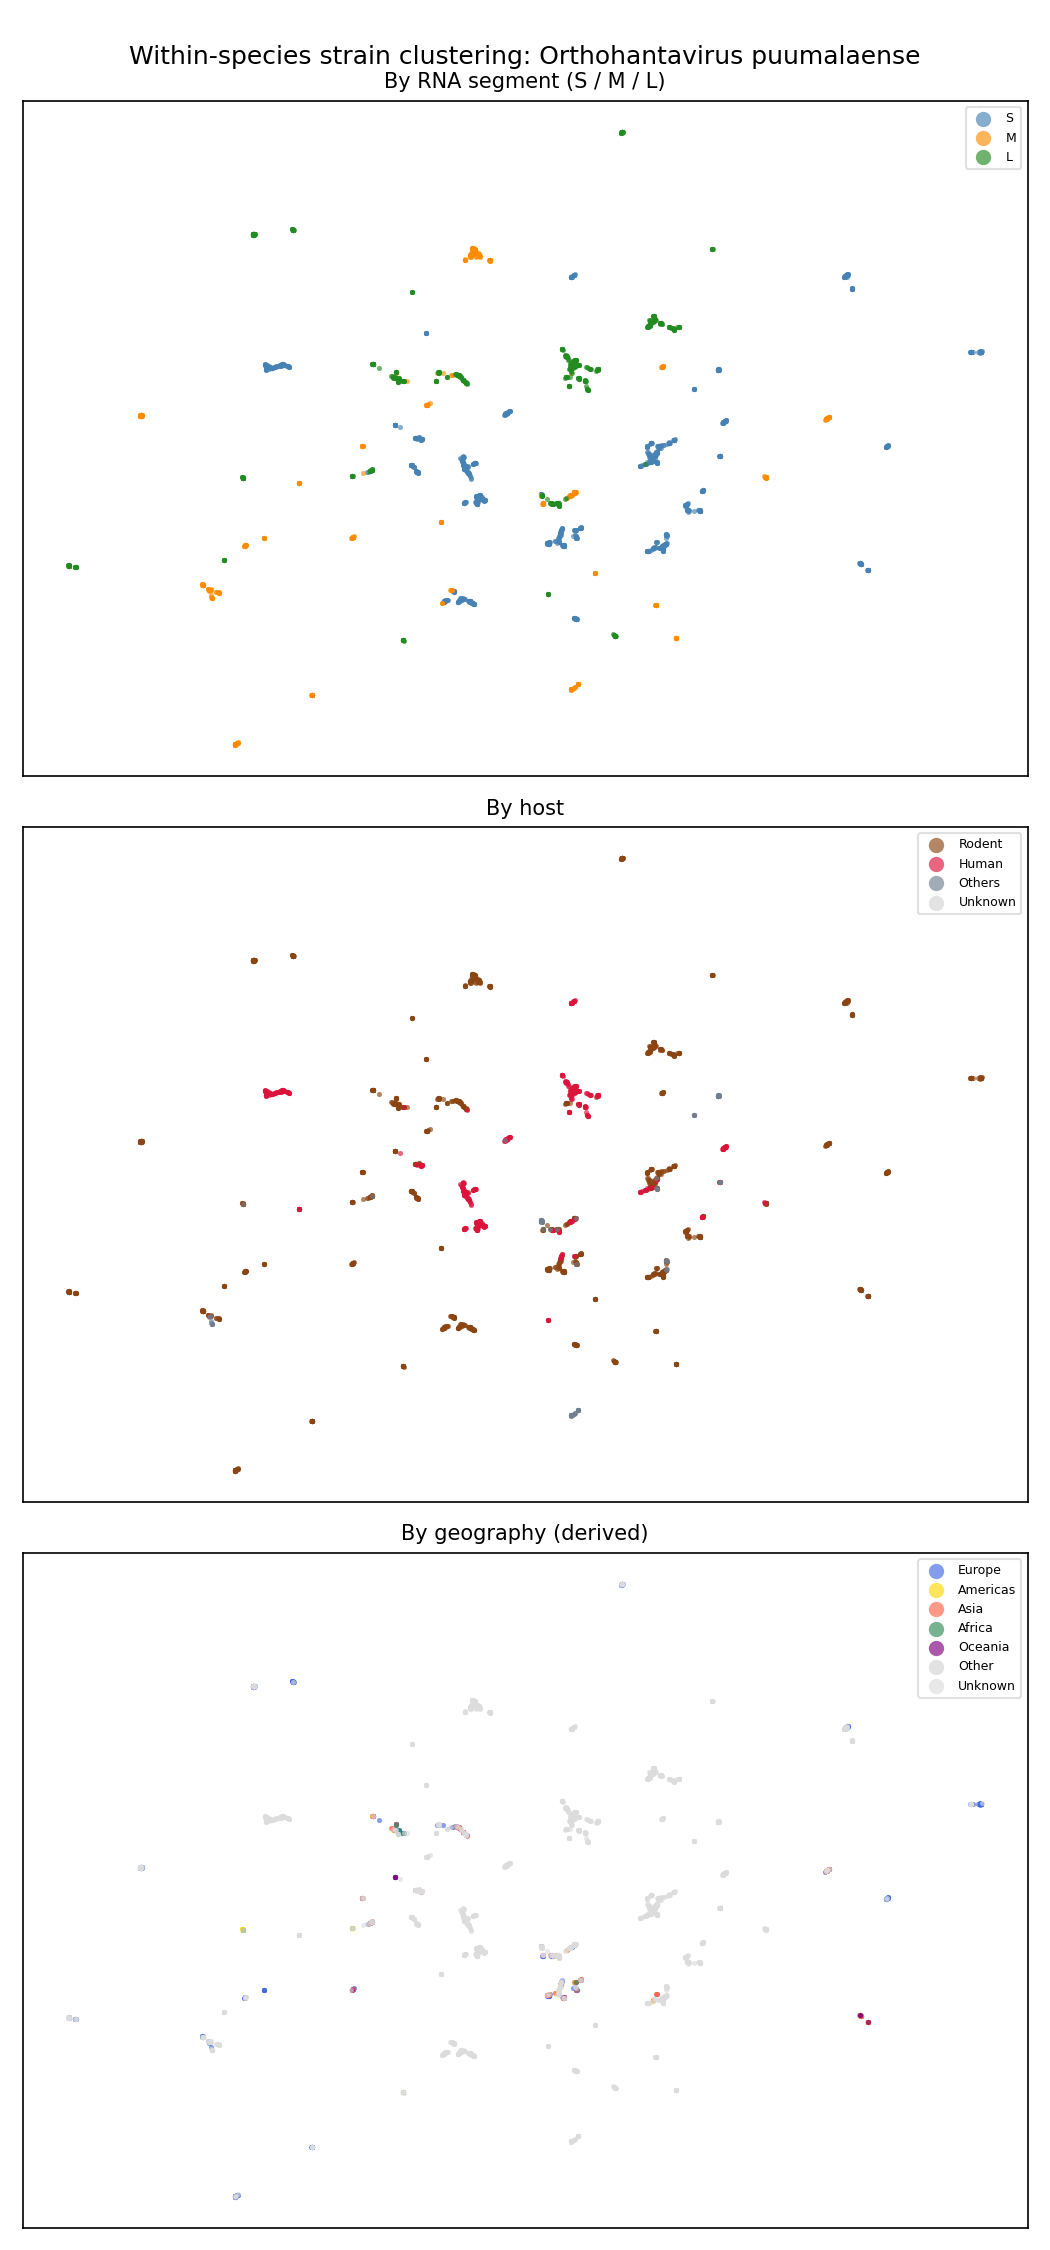
\includegraphics[width=\linewidth,height=0.6\textheight,keepaspectratio]{umap_Orthohantavirus_puumalaense.png}
\caption{UMAP intra-spesies \emph{O.\ puumalaense} (atas-bawah:
segmen / inang / geografi).}
\label{fig:umap-puumala}
\end{figure}

% =============================================================================
\section{Kesimpulan}\label{sec:conclusion}
% =============================================================================

Penelitian ini menyajikan HantaBERT, sebuah model multi-task hasil
\emph{fine-tuning} DNABERT-2 untuk klasifikasi spesies, inang, dan asal
geografis sekuens hantavirus dalam satu \emph{forward pass}. Skema
\emph{bottleneck} bersama, \emph{loss} multi-task berbobot, dan
strategi pelatihan ramah memori (AMP fp16, \emph{grad accum}, LR
diferensial) menghasilkan akurasi 96{,}7\%/91{,}4\%/80{,}5\% pada set uji
terpisah, menjawab \textbf{RQ1} secara afirmatif. \emph{Embedding}
768-d yang muncul dari pelatihan tidak hanya membentuk klaster lineage
(\textbf{RQ2}) tetapi juga substruktur per segmen genom ($S$/$M$/$L$)
yang konsisten dengan biologi virus (\textbf{RQ3}). Secara objektif,
kontribusi ini menyediakan basis komputasi yang ringkas untuk triase
sekuens hantavirus baru: klasifikasi multi-atribut + representasi
visualisasi-siap dengan satu model. Sebagai pelengkap kontribusi
\emph{engineering}, model di-\emph{deploy} di balik antarmuka web
publik (FastAPI + frontend statis HTML/JS) yang menerima sekuens
DNA/RNA atau berkas FASTA dan mengembalikan prediksi probabilistik per tugas
beserta peta geografis interaktif.

Arah pekerjaan lanjutan: (i) memperluas konteks melampaui 512 token
agar segmen $L$ panjang tidak ter-truncate; (ii) kepala kalibrasi
probabilitas (\emph{temperature}/\emph{Platt scaling}) untuk estimasi
ketidakpastian yang dapat diandalkan dalam surveilans; (iii)
\emph{ensemble} lintas segmen genom saat ketiga segmen dari satu isolat
tersedia; (iv) eksplorasi DNABERT-S sebagai \emph{backbone} alternatif
karena fungsi tujuan pra-pelatihannya \emph{species-aware}.

% =============================================================================
\begin{thebibliography}{99}

\bibitem{Zhou2023DNABERT2}
Z. Zhou, Y. Ji, W. Li, P. Dutta, R. Davuluri, dan H. Liu,
``DNABERT-2: Efficient foundation model and benchmark for multi-species
genome,'' \emph{arXiv preprint} arXiv:2306.15006, 2023.

\bibitem{Zhou2024DNABERTS}
Z. Zhou, W. Wu, H. Ho, J. Wang, L. Shi, R. V. Davuluri, Z. Wang, dan H. Liu,
``DNABERT-S: Learning species-aware DNA embedding with genome foundation
models,'' \emph{arXiv preprint} arXiv:2402.08777, 2024.

\bibitem{Ji2021DNABERT}
Y. Ji, Z. Zhou, H. Liu, dan R. V. Davuluri,
``DNABERT: pre-trained bidirectional encoder representations from
transformers model for DNA-language in genome,''
\emph{Bioinformatics}, vol. 37, no. 15, hlm. 2112-2120, 2021.

\bibitem{Devlin2019BERT}
J. Devlin, M.-W. Chang, K. Lee, dan K. Toutanova,
``BERT: Pre-training of deep bidirectional transformers for language
understanding,'' dalam \emph{Proc. NAACL-HLT}, 2019, hlm. 4171-4186.

\bibitem{Caruana1997MTL}
R. Caruana, ``Multitask learning,'' \emph{Machine Learning}, vol. 28,
hlm. 41-75, 1997.

\bibitem{McInnes2018UMAP}
L. McInnes, J. Healy, dan J. Melville,
``UMAP: Uniform manifold approximation and projection for dimension
reduction,'' \emph{arXiv preprint} arXiv:1802.03426, 2018.

\bibitem{Wolf2020Transformers}
T. Wolf \emph{et al.},
``Transformers: State-of-the-art natural language processing,'' dalam
\emph{Proc. EMNLP: System Demonstrations}, 2020, hlm. 38-45.

\bibitem{Paszke2019PyTorch}
A. Paszke \emph{et al.},
``PyTorch: An imperative style, high-performance deep learning library,''
dalam \emph{Proc. NeurIPS}, 2019.

\bibitem{Pedregosa2011Sklearn}
F. Pedregosa \emph{et al.},
``Scikit-learn: Machine learning in Python,''
\emph{J. Mach. Learn. Res.}, vol. 12, hlm. 2825-2830, 2011.

\bibitem{Loshchilov2019AdamW}
I. Loshchilov dan F. Hutter,
``Decoupled weight decay regularization,'' dalam \emph{Proc. ICLR}, 2019.

\end{thebibliography}

\end{document}
